\documentclass[fleqn]{article}
\oddsidemargin 0.0in
\textwidth 6.0in
\thispagestyle{empty}
\usepackage{import}
\usepackage{amsmath}
\usepackage{graphicx}
\usepackage[english]{babel}
\usepackage[utf8x]{inputenc}
\usepackage{float}
\usepackage[colorinlistoftodos]{todonotes}

\definecolor{hwColor}{HTML}{AD53BA}

\begin{document}

  \begin{titlepage}

    \newcommand{\HRule}{\rule{\linewidth}{0.5mm}} % Defines a new command for the horizontal lines, change thickness here

    \center % Center everything on the page
    


    \textsc{\LARGE Arizona State University}\\[1.5cm] % Name of your university/college

    \textsc{\LARGE Physics III }\\[1.5cm] % Major heading such as course name


    \begin{figure}
      
\includegraphics[width=\linewidth]{asu.png}
    \end{figure}


    \HRule \\[0.4cm]
    { \huge \bfseries Homework 6}\\[0.4cm] 
    \HRule \\[1.5cm]
    
    \textbf{Behnam Amiri}

    \bigbreak

    \textbf{Prof: David Smith}

    \bigbreak


    \textbf{{\large \today}\\[2cm]}

    \vfill % Fill the rest of the page with whitespace

  \end{titlepage}

  \begin{enumerate}
    \item Figure 34-33 shows a small lightbulb suspended at distance $d_1=250 cm$ above the surface of the water in a swimming pool where the water depth is $d_2=200 cm$ The bottom of the pool is a large mirror. How far below the mirror surface is the image of the bulb? (Hint: Assume that the rays are close to a vertical axis through the bulb, and use the small-angle approximation in which $sin\theta \approx tan \theta \approx \theta $.

    \textcolor{hwColor}{
      Step 1: Refraction at air-water surface \\
      $\dfrac{n_1}{p_1}+\dfrac{n_2}{i_1}=\dfrac{n_2-n_1}{r_1}$ where $n_1=1$ , $n_2=1.33$, $p_1=d_1$ and $r_1=\infty$ \\
      $\dfrac{n_1}{p_1}+\dfrac{n_2}{i_1}=0 \Longrightarrow i_1=-\dfrac{n_2}{n_1}p_1$ \\
      $i_1=-\dfrac{1.33}{1}(250) \rightarrow i_1=-332.5$ cm \\
    }

    \textcolor{hwColor}{
      \rule{15cm}{0.4pt}
    }

    \textcolor{hwColor}{
      Step 2: Use $i_1$ as object for reflection for mirror. \\
      $i_2=-p_2$ and $p_2=|i_1|+d_2$ \\
      $|p_2|=|i_1|+d_2=|-332.5|+200 \rightarrow p_2=532.5$ cm \\
    }

    \textcolor{hwColor}{
      \rule{15cm}{0.4pt}
    }

    \textcolor{hwColor}{
      Step 3: Use $I_2$ as object for reflection at water-air surface. \\
      $\dfrac{n_2}{p_3}+\dfrac{n_1}{i_3}=\dfrac{n_1-n_2}{r_1}$ where $r_1=\infty$ \\
      $i_3=-\dfrac{n_1}{n_2}p_3$ and $p_3=|i_2|+200 \rightarrow |p_3|=732.5$ cm \\
      $i_3=-\dfrac{1}{1.33}(732.5)=−550.751$ cm \\
      \bigbreak
      And this is how far below the mirror surface the image of the bulb is: \\
      $d_3=|i_3|-d_2=550.751-200 \Longrightarrow d_3=350.751$ cm
    }

    \begin{figure}[H]
      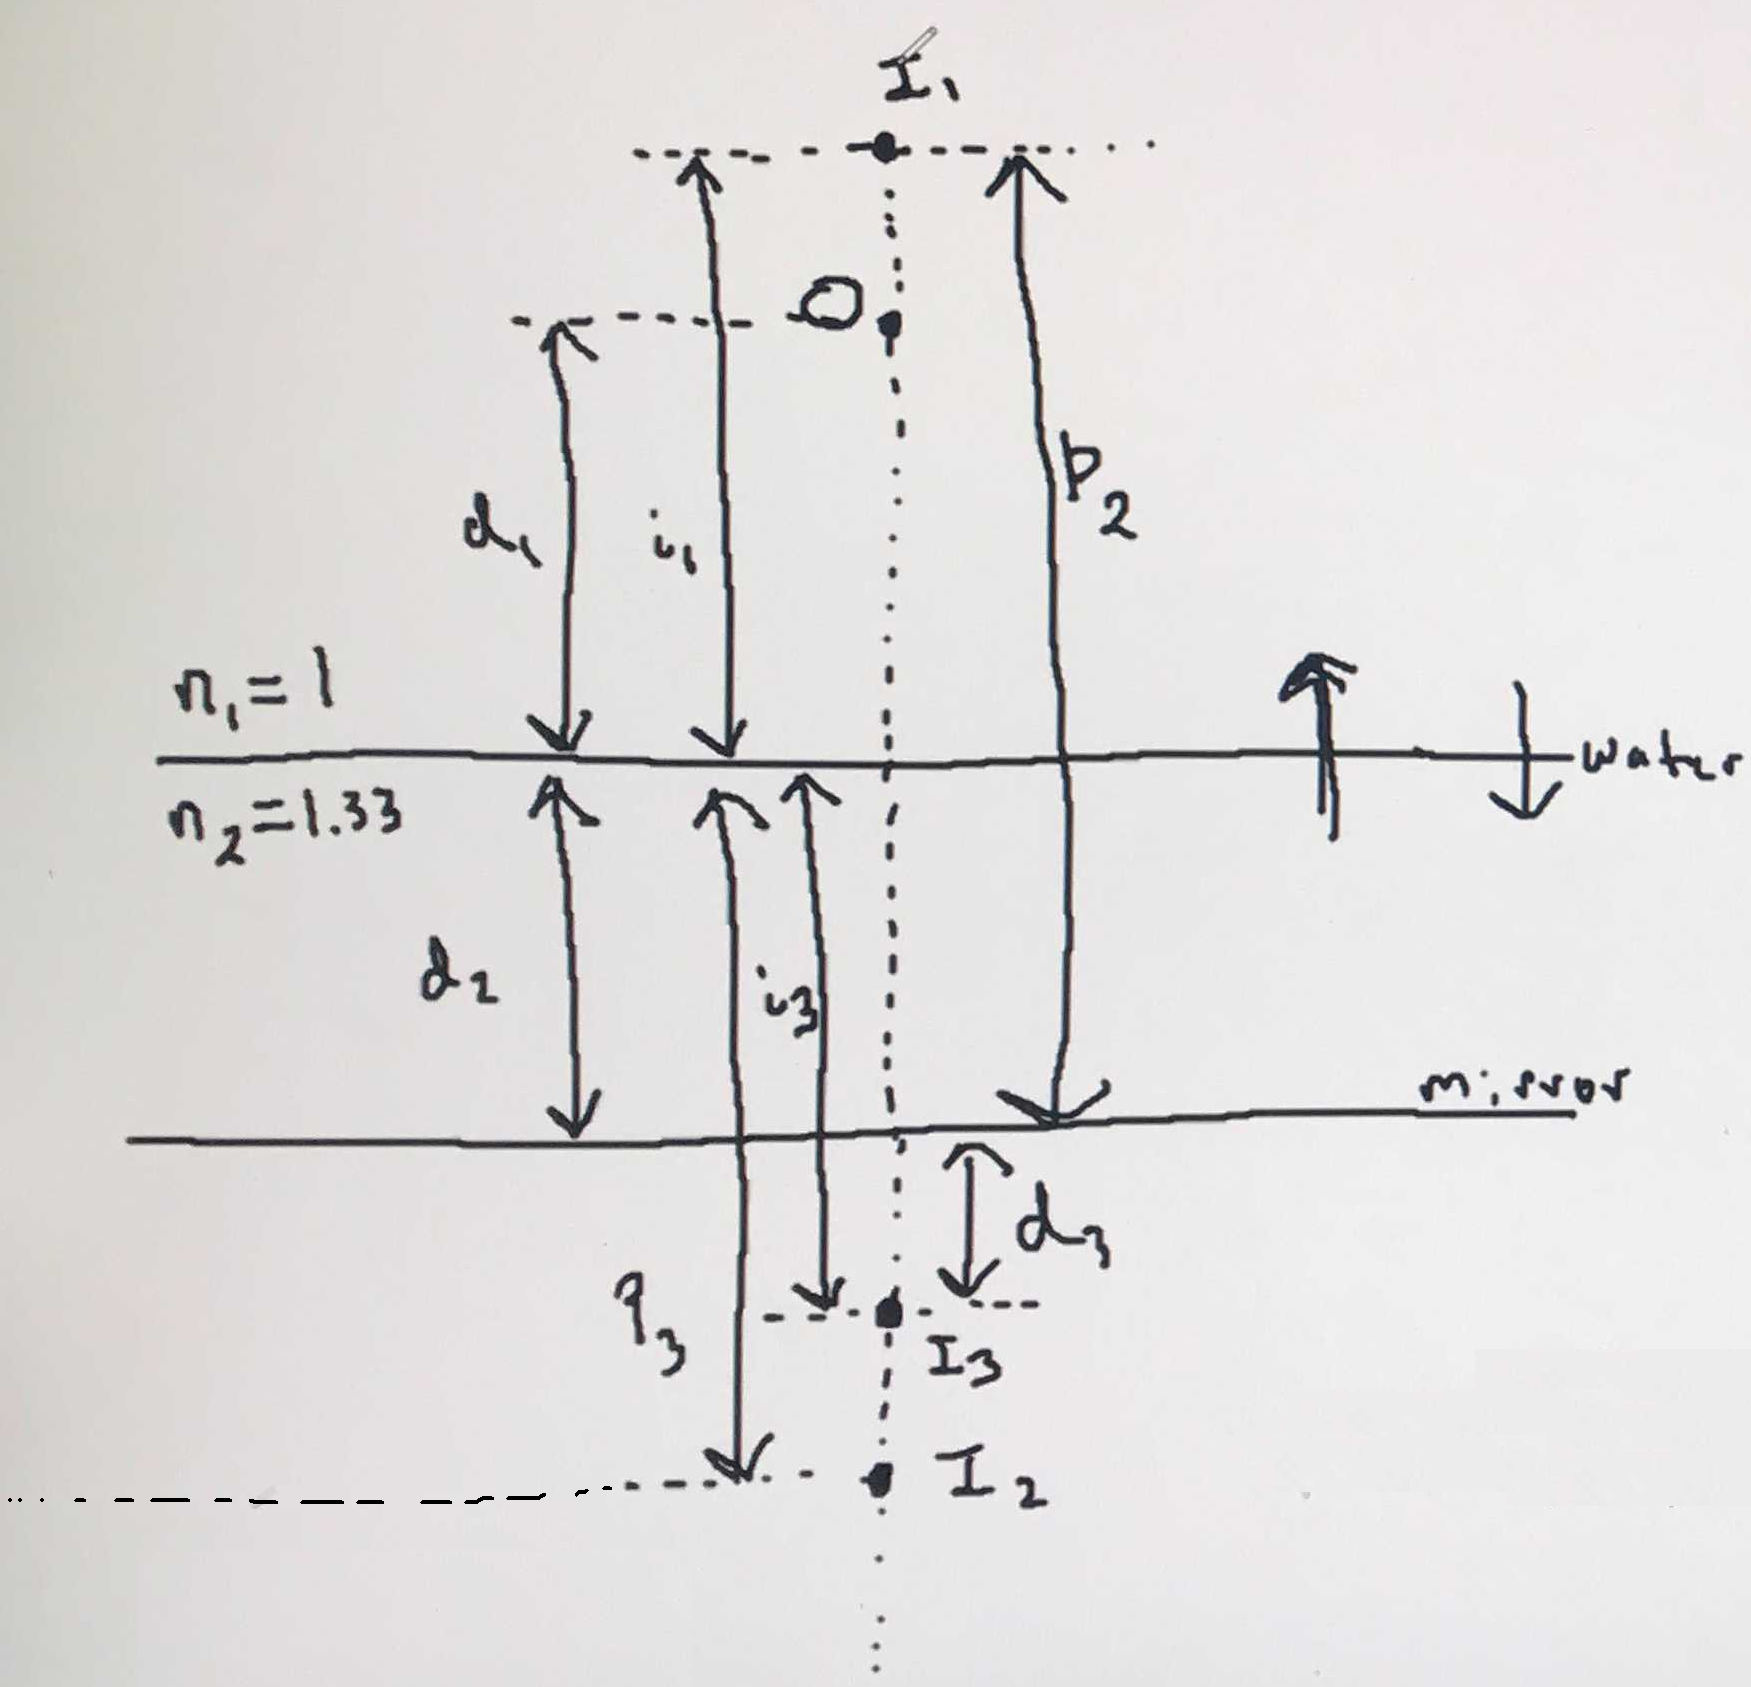
\includegraphics[width=\linewidth]{figure.png}
    \end{figure}

    \item A concave shaving mirror has a radius of curvature of 35.0 cm. It is positioned so that the (upright) image of a man’s face is 2.50 times the size of the face. How far is the mirror from the face?

      \textcolor{hwColor}{
        $
          m=-\dfrac{i}{p}
        $ 
        and for the spherical mirror
        \\
        $
          \dfrac{1}{p}+\dfrac{1}{i}=\dfrac{2}{r}
        $ 
        by a doing a little algebra
        $
          \dfrac{1}{p}-\dfrac{1}{mp}=\dfrac{2}{r}
        $
        \\
        $
          p=\dfrac{r(m-1)}{2m}=\dfrac{35 cm(2.5-1)}{2(2.5)}
        $
        \\
        $
          \rightarrow p=10.5 cm
        $
      }

    \item 23, 29 22 More mirrors. Object O stands on the central axis of a spherical or plane mirror. For this situation, each problem in Table 34-4 refers to (a) the type of mirror, (b) the focal distance f, (c) the radius of curvature r, (d) the object distance p, (e) the image distance i, and (f) the lateral magnification m. (All distances are in centimeters.) It also refers to whether (g) the image is real (R) or virtual (V), (h) inverted (I) or noninverted (NI) from O, and (i) on the same side of the mirror as object O or on the opposite side. Fill in the missing information. Where only a sign is missing, answer with the sign.
    
    \textcolor{hwColor}{
      17:  \\
      a) Concave \\
      b) $f=20$ \\
      c) $r=2f=2(20)=40$ cm \\
      d) $p=10$ cm \\
      e) $\dfrac{1}{f}=\dfrac{1}{p}+\dfrac{1}{i} \rightarrow \dfrac{1}{i}=\dfrac{1}{f}-\dfrac{1}{p}=\dfrac{1}{20}-\dfrac{1}{10} \rightarrow i=-20$ cm \\
      f) $m=-\dfrac{i}{p}=-\dfrac{-20}{10}=2$ \\
      g) The image is virtual since i is negative. \\
      h) m is positive, therefore the image is noninverted. \\
      i) i is negative, hence the image is on the opposite side. \\
    }

    \textcolor{hwColor}{
      \rule{15cm}{0.4pt}
    }

    \textcolor{hwColor}{
      18: \\
      $p=24$ cm, $m=0.50$ and Inverted\\
      $i=-pm=-(24 cm)(0.50)=-12$ cm \\
      $\dfrac{1}{f}=\dfrac{1}{p}+\dfrac{1}{i}=\dfrac{1}{24}+\dfrac{1}{-12} \rightarrow f=-24$ cm \\
      $r=2f=2(-24)=-48$ cm \\
      a) Convex \\
      b) $f=-24$ cm \\
      c) $r=-48$ cm \\
      d) $p=24$ cm \\
      e) $i=-12$ cm \\
      f) $m=0.50$ \\
      g) The image is virtual since i is negative. \\
      h) m is positive, therefore the image is noninverted. \\
      i) i is negative, hence the image is on the opposite side. \\
    }

    \textcolor{hwColor}{
      \rule{15cm}{0.4pt}
    }

    \textcolor{hwColor}{
      19: \\
      $r=-40$ cm, $i=-10$ cm\\
      $f=\dfrac{1}{2}r=\dfrac{1}{2}(-40)=-20$ cm. \\
      $\dfrac{1}{f}=\dfrac{1}{p}+\dfrac{1}{i} \rightarrow \dfrac{1}{p}=\dfrac{1}{f}-\dfrac{1}{i}=\dfrac{1}{-20}-\dfrac{1}{-10}=\dfrac{1}{20}$ \\
      $m=\dfrac{-i}{p}=-\dfrac{-10}{20}=0.50$
      a) Convex \\
      b) $f=-20$ cm \\
      c) $r=-40$ cm \\
      d) $p=20$ cm \\
      e) $i=-10$ cm \\
      f) $m=0.50$ \\
      g) The image is virtual since i is negative. \\
      h) m is positive, therefore the image is noninverted. \\
      i) i is negative, hence the image is on the opposite side. \\
    }

    \textcolor{hwColor}{
      \rule{15cm}{0.4pt}
    }

    \textcolor{hwColor}{
      20: \\
      $p=40$ cm and $m=-0.70$ \\
      $i=-pm=-(40)(-0.70)=28$ \\
      $r=2f=2(\dfrac{280}{17})=\dfrac{560}{17}$ \\
      a) Concave \\
      b) $f=\dfrac{280}{17}$ cm \\
      c) $r=\dfrac{560}{17}$ cm \\
      d) $p=40$ cm \\
      e) $i=28$ cm \\
      f) $m=-0.70$ \\
      g) The image is real since i is positive. \\
      h) m is negative, therefore the image is inverted. \\
      i) i is positive, hence the image is on the same side. \\
    }

    \textcolor{hwColor}{
      \rule{15cm}{0.4pt}
    }

    \textcolor{hwColor}{
      21: \\
      $f=20$ cm and $p=30$ cm \\
      $\dfrac{1}{f}=\dfrac{1}{p}+\dfrac{1}{i} \rightarrow \dfrac{1}{i}=\dfrac{1}{f}-\dfrac{1}{p}=\dfrac{1}{20}-\dfrac{1}{30}=\dfrac{1}{60}$ \\
      $r=2f=2(20)=40$ cm \\
      a) Concave \\
      b) $f=20$ cm \\
      c) $r=40$ cm \\
      d) $p=30$ cm \\
      e) $i=60$ cm \\
      f) $m=-3$ \\
      g) The image is real since i is positive. \\
      h) m is negative, therefore the image is inverted. \\
      i) i is positive, hence the image is on the same side. \\
    }

    \textcolor{hwColor}{
      \rule{15cm}{0.4pt}
    }

    \textcolor{hwColor}{
      22: \\
      $f=20$ cm and $m=0.10$ \\
      $r=2f=2(20)=40$ cm \\
      $i=-0.10p$ \\
      $\dfrac{1}{f}=\dfrac{1}{p}+\dfrac{1}{i} \rightarrow \dfrac{1}{20}=\dfrac{1}{p}+\dfrac{1}{-0.10p}$ \\
      $p=-180$ cm \\
      $i=-0.10(-180)=18$ cm \\
      $m=-\dfrac{i}{p}=-\dfrac{18}{180}=0.1$ \\
      a) Concave \\
      b) $f=20$ cm \\
      c) $r=40$ cm \\
      d) $p=-180$ cm \\
      e) $i=18$ cm \\
      f) $m=0.10$ \\
      g) The image is real since i is positive. \\
      h) m is positive, therefore the image is noninverted. \\
      i) i is positive, hence the image is on the same side. \\
    }

    \textcolor{hwColor}{
      \rule{15cm}{0.4pt}
    }

    \textcolor{hwColor}{
      23: \\
      $f=30$ cm and $m=0.20$ \\
      $r=2f=2(30)=60$ cm \\
      $i=-pm=-0.20p$ \\
      $\dfrac{1}{f}=\dfrac{1}{p}+\dfrac{1}{i} \rightarrow \dfrac{1}{30}=\dfrac{1}{p}+\dfrac{1}{-0.20p} \Longrightarrow p=-120$ cm \\
      $i=-0.20(-120)=24$ cm \\
      a) Concave \\
      b) $f=30$ cm \\
      c) $r=60$ cm \\
      d) $p=-120$ cm \\
      e) $i=24$ cm \\
      f) $m=0.20$ \\
      g) The image is real since i is positive. \\
      h) m is positive, therefore the image is noninverted. \\
      i) i is positive, hence the image is on the same side. \\
    }

    \textcolor{hwColor}{
      \rule{15cm}{0.4pt}
    }

    \textcolor{hwColor}{
      24: \\
      $p=60$ cm and $m=-0.50$ \\
      $i=-pm=-(60)(-0.50)=30$ cm \\
      $\dfrac{1}{f}=\dfrac{1}{p}+\dfrac{1}{i}=\dfrac{1}{60}+\dfrac{1}{30} \Longrightarrow f=20$ cm \\
      $r=2f=2(20)=40$ cm \\
      a) Concave \\
      b) $f=20$ cm \\
      c) $r=40$ cm \\
      d) $p=60$ cm \\
      e) $i=30$ cm \\
      f) $m=-0.50$ \\
      g) The image is real since i is positive. \\
      h) m is negative, therefore the image is inverted. \\
      i) i is positive, hence the image is on the same side. \\
    }

    \textcolor{hwColor}{
      \rule{15cm}{0.4pt}
    }

    \textcolor{hwColor}{
      25: \\
      $p=30$ cm and $m=0.40$ \\
      $i=-pm=(-30)(0.40)=-12$ cm \\
      $\dfrac{1}{f}=\dfrac{1}{p}+\dfrac{1}{i}=\dfrac{1}{30}+\dfrac{1}{-12} \Longrightarrow f=-20$ cm \\
      $r=2f=2(-20)=-40$ cm \\
      a) Convex \\
      b) $f=-20$ cm \\
      c) $r=-40$ cm \\
      d) $p=30$ cm \\
      e) $i=-12$ cm \\
      f) $m=0.40$ \\
      g) The image is virtual since i is negative. \\
      h) m is positive, therefore the image is noninverted. \\
      i) i is negative, hence the image is on the opposite side. \\
    }


    \textcolor{hwColor}{
      \rule{15cm}{0.4pt}
    }

    \textcolor{hwColor}{
      26: \\
      $f=20$ and $p=60$ \\
      $\dfrac{1}{f}=\dfrac{1}{p}+\dfrac{1}{i} \rightarrow \dfrac{1}{i}=\dfrac{1}{f}-\dfrac{1}{p}=\dfrac{1}{20}-\dfrac{1}{60} \Longrightarrow i=30$ cm \\
      $m=-\dfrac{i}{p}=-\dfrac{30}{60}=-0.50$ \\
      $r=2f=2(20)=40$ cm \\
      a) Concave \\
      b) $f=20$ cm \\
      c) $r8=40$ cm \\
      d) $p=60$ cm \\
      e) $i=30$ cm \\
      f) $m=-0.50$ \\
      g) The image is real since i is positive. \\
      h) m is negative, therefore the image is inverted. \\
      i) i is positive, hence the image is on the same side. \\
    }

    \textcolor{hwColor}{
      \rule{15cm}{0.4pt}
    }

    \textcolor{hwColor}{
      27: \\
      $f=-30$ cm and $i=-15$ cm \\
      $r=2f=2(-30)=-60$ cm \\
      $\dfrac{1}{f}=\dfrac{1}{p}+\dfrac{1}{i} \rightarrow \dfrac{1}{p}=\dfrac{1}{f}-\dfrac{1}{i}=\dfrac{1}{-30}-\dfrac{1}{-15}=-\dfrac{1}{-30} \Longrightarrow p=30$ cm \\
      $m=-\dfrac{i}{p}=-\dfrac{-15}{30}=0.50$ \\
      a) Convex \\
      b) $f=-30$ cm \\
      c) $r=-60$ cm \\
      d) $p=30$ cm \\
      e) $i=-15$ cm \\
      f) $m=0.50$ \\
      g) The image is virtual since i is negative. \\
      h) m is positive, therefore the image is noninverted. \\
      i) i is negative, hence the image is on the opposite side. \\
    }

    \textcolor{hwColor}{
      \rule{15cm}{0.4pt}
    }

    \textcolor{hwColor}{
      28: \\
      $p=10$ cm and $m=1$ \\
      $i=-pm=-10(1.0)=-10$ \\
      $\dfrac{1}{f}=\dfrac{1}{p}+\dfrac{1}{i}=\dfrac{1}{10}+\dfrac{1}{-10}=0$ \\
      a) By convention when both $f$ and $r$ are positive, it is concave and when both $f$ and $r$ are negative. Therefore, it is neither concave nor convex.  \\
      b) $f=0$ cm \\
      c) $r=0$ cm \\
      d) $p=10$ cm \\
      e) $i=-10$ cm \\
      f) $m=1$ \\
      g) The image is virtual since i is negative. \\
      h) m is positive, therefore the image is noninverted. \\
      i) i is negative, hence the image is on the opposite side. \\
    }

    \textcolor{hwColor}{
      \rule{15cm}{0.4pt}
    }

    \textcolor{hwColor}{
      29: \\
      $r=40$ cm and $i=4$ cm \\
      $f=\dfrac{1}{2}r=\dfrac{1}{2}(40)=20$ cm but since we are told the mirror is convex then $f=-20$ cm \\
      $\dfrac{1}{f}=\dfrac{1}{p}+\dfrac{1}{i} \rightarrow \dfrac{1}{p}=\dfrac{1}{f}-\dfrac{1}{i}=\dfrac{1}{-20}-\dfrac{1}{4}=\dfrac{6}{-20} \Longrightarrow p=-\dfrac{10}{3}$ \\
      $m=-\dfrac{i}{p}=-\dfrac{-4}{-\dfrac{10}{3}} \Longrightarrow m=1.2$ \\
      a) Convex \\
      b) $f=-20$ cm \\
      c) $r=-40$ cm \\
      d) $p=-\dfrac{10}{3}$ cm \\
      e) $i=4$ cm \\
      f) $m=1.2$ \\
      g) The image is real since i is positive. \\
      h) m is positive, therefore the image is noninverted. \\
      i) i is positive, hence the image is on the same side. \\
    }


    \item In Fig. 34-37, a beam of parallel light rays from a laser is incident on a solid transparent sphere of index of refraction n. (a) If a point image is produced at the back of the sphere, what is the index of refraction of the sphere? (b) What index of refraction, if any, will produce a point image at the center of the sphere?

    \textcolor{hwColor}{
      We have the following for a spherical refracting surfaces.\\
      (a): \\
      $\dfrac{n_1}{p}+\dfrac{n_2}{i}=\dfrac{n_2-n_1}{r}$ \\
      $\dfrac{1}{\infty}+\dfrac{n}{2r}=\dfrac{n-1}{r} \Longrightarrow n=2$ \\
      \bigbreak
      (b): \\
      $\dfrac{1}{\infty}+\dfrac{n}{r}=\dfrac{n-1}{r} \rightarrow \dfrac{n}{r}=\dfrac{n-1}{r}$ \\
      \\
      This result can not be true, hence it is not doable $(\dfrac{n}{r} \neq \dfrac{n-1}{r})$.
    }
    
    \item A movie camera with a (single) lens of focal length 75 mm takes a picture of a person standing 27 m away. If the person is 180 cm tall, what is the height of the image on the film?

    \textcolor{hwColor}{
      We know that $m=\dfrac{h_i}{h_p}$ and $m=-\dfrac{i}{p}$ \\
      The height of the image on the film is $h_i=m.h_p$ \\
      $\dfrac{1}{f}=\dfrac{1}{p}+\dfrac{1}{i} \rightarrow \dfrac{1}{i}=\dfrac{1}{f}-\dfrac{1}{p} \Longrightarrow i=\dfrac{fp}{p-f}$ \\
      $m=\dfrac{-i}{p}=-\dfrac{\dfrac{fp}{p-f}}{p}=\dfrac{-f}{p-f}$ \\
      $h_i=(\dfrac{-f}{p-f}).h_p=\dfrac{-(75\times10^-3)\times 1.8}{27-(75\times10^-3)}\approx -5.013 mm$ \\
      \bigbreak
      $\Longrightarrow |h_i|\approx 5.013 mm$
    }

    \item In Fig. 34-43, a real inverted image I of an object O is formed by a certain lens (not shown); the object–image separation is d=40.0 cm, measured along the central axis of the lens. The image is just half the size of the object. (a) What kind of lens must be used to produce this image? (b) How far from the object must the lens be placed? (c) What is the focal length of the lens?

    \textcolor{hwColor}{
      (a): It is gotta be a concave lens since the image is on the other side. \\
      (b): \\
      We know $p+i=40$ cm and $m=-\dfrac{1}{2}$ \\
      $i=-mp=-(-\dfrac{1}{2})p=\dfrac{1}{2}p$ \\
      $p+i=40 \rightarrow p=40-i=40-\dfrac{1}{2}p \Longrightarrow p=\dfrac{80}{3}$ cm \\
      (c): \\
      $\dfrac{1}{f}=\dfrac{1}{p}+\dfrac{1}{i}=\dfrac{1}{\dfrac{80}{3}}+\dfrac{1}{\dfrac{80}{6}} \Longrightarrow f\approx 8.88$ cm.
    }
    
    \item 75, 77 78 More lenses. Object O stands on the central axis of a thin symmetric lens. For this situation, each problem in Table 34-8 refers to (a) the lens type, converging (C) or diverging (D), (b) the focal distance f, (c) the object distance p, (d) the image distance i, and (e) the lateral of its focal points (the proper sign of the focal distance is not indicated). Find (a) the image distance i2 for the image produced by lens 2 (the final image produced by the system) and (b) the overall lateral magnification M for the system, including signs. Also, determine whether the final image is (c) real (R) or virtual (V), (d) inverted (I) from object O or noninverted (NI), and (e) on the same side of lens 2 as object O or on the opposite side.

    \textcolor{hwColor}{
      69: \\
      a)  \\
      b)  \\
      c)  \\
      d)  \\
      e)  \\
    }

    \textcolor{hwColor}{
      \rule{15cm}{0.4pt}
    }

    \textcolor{hwColor}{
      70: \\
      a)  \\
      b)  \\
      c)  \\
      d)  \\
      e)  \\
    }

    \textcolor{hwColor}{
      \rule{15cm}{0.4pt}
    }

    \textcolor{hwColor}{
      71: \\
      a)  \\
      b)  \\
      c)  \\
      d)  \\
      e)  \\
    }

    \textcolor{hwColor}{
      \rule{15cm}{0.4pt}
    }

    \textcolor{hwColor}{
      72: \\
      a)  \\
      b)  \\
      c)  \\
      d)  \\
      e)  \\
    }

    \textcolor{hwColor}{
      \rule{15cm}{0.4pt}
    }

    \textcolor{hwColor}{
      73: \\
      a)  \\
      b)  \\
      c)  \\
      d)  \\
      e)  \\
    }

    \textcolor{hwColor}{
      \rule{15cm}{0.4pt}
    }

    \textcolor{hwColor}{
      74: \\
      a)  \\
      b)  \\
      c)  \\
      d)  \\
      e)  \\
    }

    \textcolor{hwColor}{
      \rule{15cm}{0.4pt}
    }

    \textcolor{hwColor}{
      75: \\
      a)  \\
      b)  \\
      c)  \\
      d)  \\
      e)  \\
    }

    \textcolor{hwColor}{
      \rule{15cm}{0.4pt}
    }

    \textcolor{hwColor}{
      76: \\
      a)  \\
      b)  \\
      c)  \\
      d)  \\
      e)  \\
    }

    \textcolor{hwColor}{
      \rule{15cm}{0.4pt}
    }


    \textcolor{hwColor}{
      77: \\
      a)  \\
      b)  \\
      c)  \\
      d)  \\
      e)  \\
    }

    \textcolor{hwColor}{
      \rule{15cm}{0.4pt}
    }

    \textcolor{hwColor}{
      78: \\
      a)  \\
      b)  \\
      c)  \\
      d)  \\
      e)  \\
    }

    \textcolor{hwColor}{
      \rule{15cm}{0.4pt}
    }

    \textcolor{hwColor}{
      79: \\
      a)  \\
      b)  \\
      c)  \\
      d)  \\
      e)  \\
    }
    
  \end{enumerate}

\end{document}
